\chapter{Results}

Our proclaimed goal for the visualization was to enable large hierarchical networks in VR. 
Therefore, we tested our application in a performance evaluation in Section \ref{sec:performanceEvaluation} and gather different user feedback in the form of a heuristic evaluation (see Section \ref{sec:heuristicEvaluation}).

\section{Performance}
\label{sec:performanceEvaluation}

Real time 3D applications need to have a constant frame rate in order to achieve a smooth experience.
For VR-based applications this is even more important as a low frame rate could lead to motion sickness. 
In our performance test we distinguish between the initial phase when the application is started until the force based layout algorithm is finished and the actual exploration phase. 
The exploration phase usually lasts for multiple minutes, while the initial phase only lasts for a maximum of 1.5 minutes.
Therefore, we assume a low performance during the layout calculation is not as critical as the exploration performance. 
The user can simply wait until the layout is completely finished before interacting with the graph.

In the performance evaluation we wanted to find out the quantity structure of the dataset. 
For an optimal VR experience the frame rate should be constant and equal to the maximum supported refresh rate of the VR headset's displays. In the case of the HTC Vive this requires us to have a consta t frame rate of 90 FPS.
Own experiments showed that 20-30 FPS is the minimum while exploring a virtual scene without being distracted.
\\
We measured the FPS directly from the visualization by adding an FPS counter on the virtual controller model during the exploration. Our setup was a desktop PC with a Ryzen 7 3700X CPU and a Radeon RX 590 GPU. 
We tested multiple datasets with different sizes, the results are shown in Table \ref{table:resultFPS}. 
In order to detect possible performance problems we tested the scaling of the nodes and links individually as good as possible.
We found out that the number of nodes scale worse than the number of links (see Figure \ref{fig:performanceNodes} and \ref{fig:performanceLinks}). 
When we assume an equal distributed graph, the number of hierarchical layers only indirectly influence the frame rate, as with an increased number of layers the number of nodes grows exponentially. 
So before the application would run into performance problems based on the number of layers, the number of nodes would be too large anyway. 
In addition, at about 6 hierarchical layers the layout algorithm becomes unstable and can not guarantee a correct hierarchical nesting anymore.
\\
While the average frame rate is not drastically reduced by the links, the frame rate seems to get more unstable. 
This was especially noticeable during the teleportation animation were the frame rate dropped on a large dataset up to 20 FPS. 
Although we do not know for sure, we assume the automated scaling reduced the frame rate quite significantly. During the animation the scale of nearly all objects in the scenes is updated on every frame.
Our data only shows a maximum of 90 FPS due to the maximum refresh panel of 90 Hz of the headset.
\\
In conclusion, with the current state of implementation the visualization can support datasets up to 1500 nodes and 3000 links depending on the hardware available.
In addition, we noticed that during the exploration the CPU and GPU utilization was not at maximum. An explanation for this could be that the application is CPU bound and further limited by a single threaded JavaScript implementation.

\begin{table}[!hbt]
    \resizebox{\textwidth}{!}{%
    \centering
    \begin{tabular}{ | c | c | c | c | c | c | }
        \hline
        \textbf{nodes} & \textbf{links} &\textbf{layers} &\textbf{layout - avg FPS} &\textbf{expl. - min FPS} &\textbf{expl. - avg FPS}\\
        \hline
        310  & 0    & 3 & 40 & 90 & 90\\ \hline
        730  & 0    & 3 & 30 & 70 & 75\\ \hline
        1100 & 0    & 3 & 20 & 55 & 60\\ \hline
        1560 & 0    & 4 & 20 & 40 & 55\\ \hline
        2343 & 0    & 5 & 10 & 30 & 35\\ \hline
        774  & 387  & 3 & 20 & 60 & 70\\ \hline
        774  & 1548 & 3 & 20 & 55 & 70\\ \hline
        774  & 3870 & 3 & 10 & 40 & 60\\ \hline
        1560 & 3120 & 4 & 5  & 25 & 45\\ \hline
        1020 & 2040 & 4 & 10 & 40 & 60\\ \hline
     \end{tabular}}
     \caption{Results from performance measurement evaluation (expl. ... exploration). Test setup: Ryzen 7 3700X + Radeon RX 590.}
     \label{table:resultFPS}
\end{table}

\begin{figure}[!hbt]
    \centering
    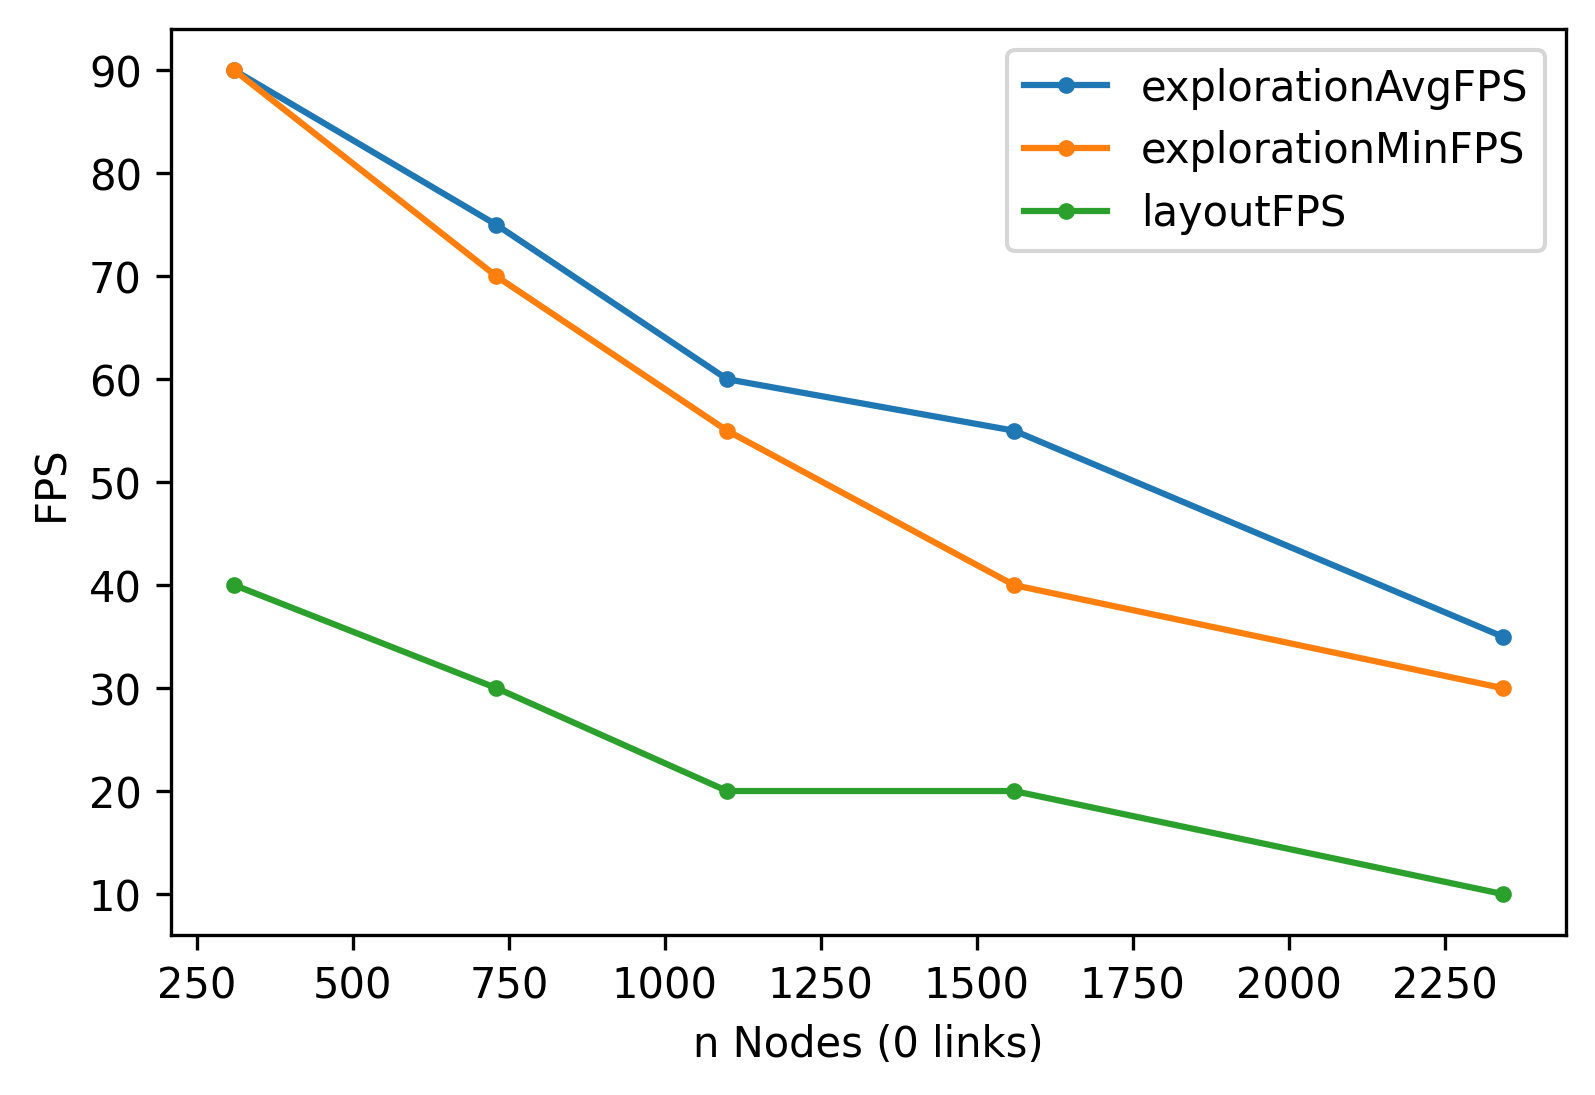
\includegraphics[width=0.75\textwidth]{graphics/performanceAnalysisNodes.png}
    \caption{Performance chart for scaling the number of nodes. To better compare the results only datasets with 0 links are shown in this graph. Increasing the number of nodes quickly leads to a performance issue.} 
    \label{fig:performanceNodes} 
\end{figure}

\begin{figure}[!hbt]
    \centering
    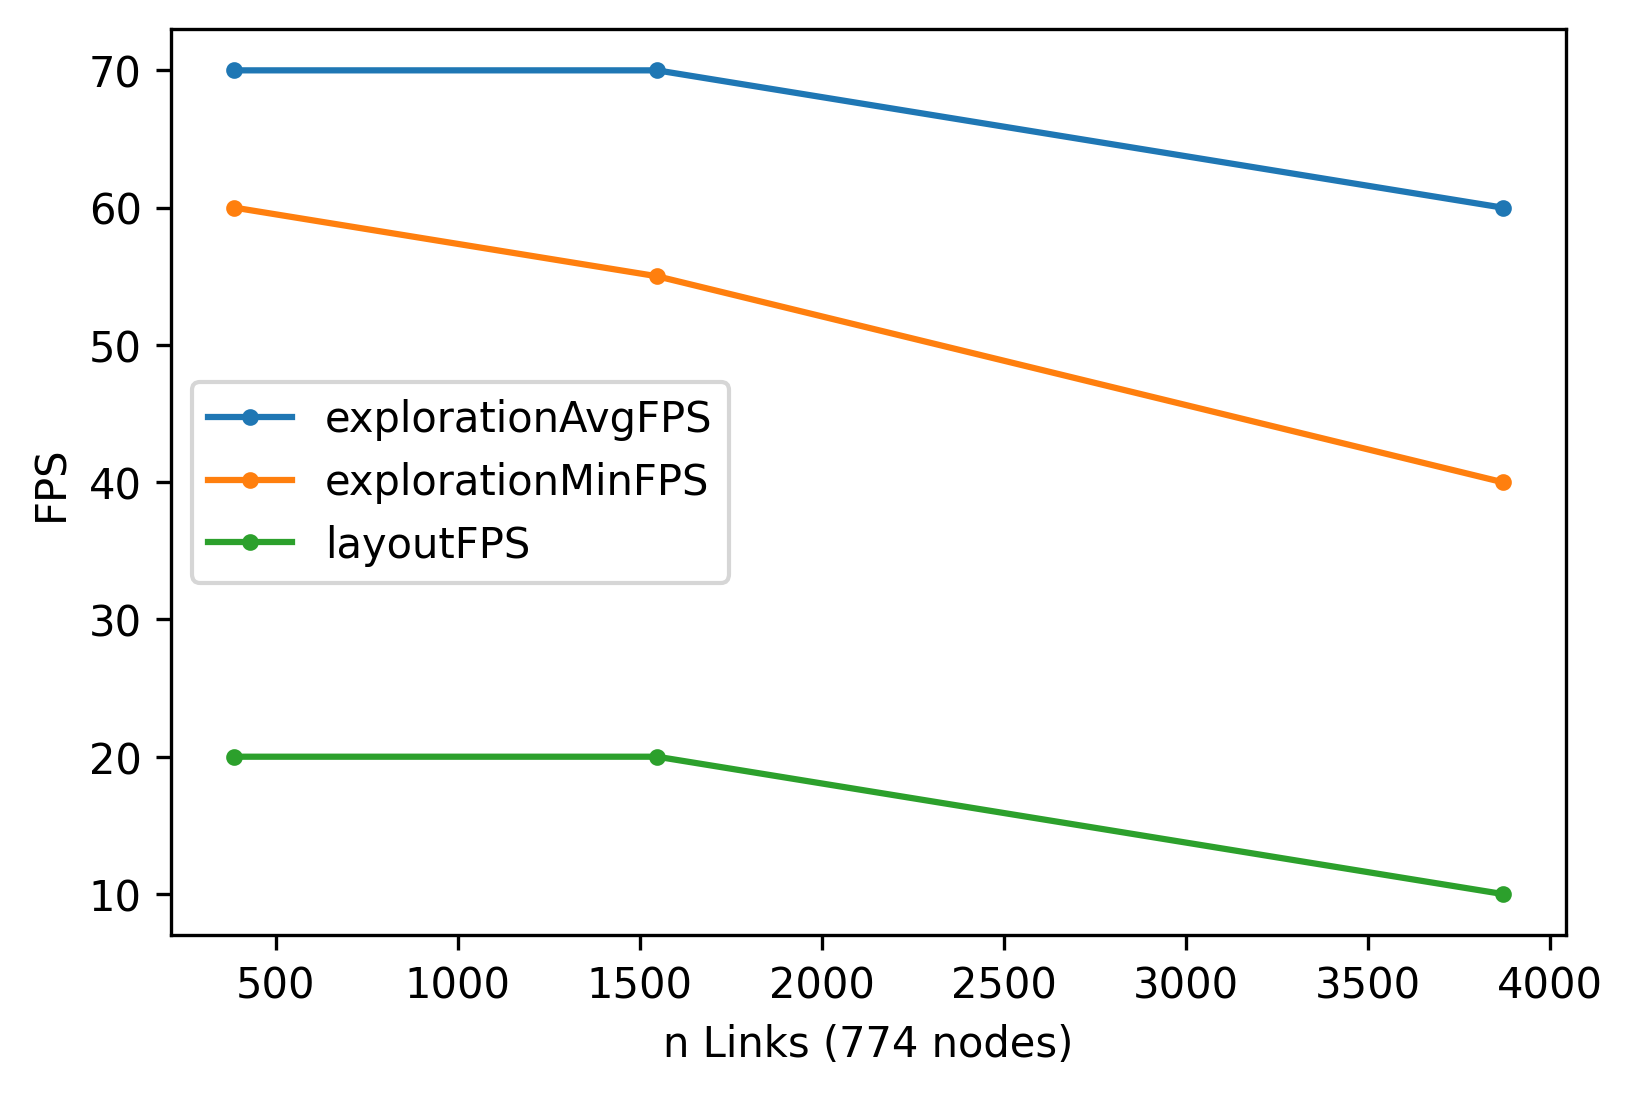
\includegraphics[width=0.75\textwidth]{graphics/performanceAnalysisLinks.png}
    \caption{Performance chart for scaling the number of links. To better compare the results only datasets with the same amount of 774 nodes are shown in this graph. In comparison to the nodes, links can be easier scaled up without impacting the performance too much.} 
    \label{fig:performanceLinks} 
\end{figure}

\subsection{Possible optimization}

To increase the overall performance the scalability for the number of nodes needs to be improved. We can separate the performance problems between GPU and CPU bottlenecks.
\\
To increase the GPU performance we already limit the draw calls by rendering the nodes with instanced buffers.
However, the number of rendered triangles is still very high. 
One improvement could be to use simpler sphere models with a lower polygon count. Implementing a technique that prevents the rendering of the small nodes which can not be seen anyway could further increase GPU performance.
\\
To increase CPU performance we have to reduce the number of tasks during each iteration of the main render loop (see Figure \ref{fig:impl_programFlow}).
A big performance issues might be the calculation of the intersected objects from ray casting by the virtual laser pointer. This could be improved by take advantage of the hierarchical layout. A ray intersection of child nodes from different parents than the one the user is currently inside is not possible anyways. Therefore, these nodes could be excluded from the ray intersection checks. 
Another improvement could be achieved by limiting the active time of the ray casting by binding the virtual laser pointer to a button that the user actively needs to hold while selecting objects. 
That would enable an improved frame rate when the user is only looking around without using the virtual laser pointer.
\\
Besides performance improvements to the techniques themselves, improving the internal data structure would also increase the performance. Based on the prior implementation we use a flat list similar to the JSON seen in Section \ref{lst:internalJSON}. With a tree data structure that directly represents the hierarchical relationships our internal algorithms could be improved as a faster access to the nodes would be possible.

\section{Heuristic Evaluation}
\label{sec:heuristicEvaluation}

The focus of this thesis was to develop a new visualization technique, this included a hierarchical layout, optimization for the use in different VR experiences and VR optimized navigation and interaction techniques.
The visualization should deliver a smooth and user-friendly visualization tool, to test the usability we gathered feedback from multiple people using an online form.
As the application just runs in the browser, we set up a hosted version \cite{thesisWebsite} with an included introduction to the topic and user instructions on how to start and interact with the visualization. The hosted version included multiple datasets with various sizes. Afterwards we invited users to participate in the evaluation and fill out the online form we prepared.
\\
Besides doing an online evaluation we also had one participant that tried our the visualization on site were we interviewed him during the exploration.
The results of the interview as well as the online forms are presented in the appropriated subsections.
\\
   
\subsection{Clarity of the visualization}
Filtering, visual clutter, hierarchical layout(intuitive?), ...

\subsection{Navigation}
Free fly, animated teleport, scaling, motion sickness.

\subsection{Interaction}
Button Mappings, Laser Pointer, 

\subsection{Performance}
Tested system and dataset